% Options for packages loaded elsewhere
\PassOptionsToPackage{unicode}{hyperref}
\PassOptionsToPackage{hyphens}{url}
%
\documentclass[
]{article}
\usepackage{amsmath,amssymb}
\usepackage{lmodern}
\usepackage{iftex}
\ifPDFTeX
  \usepackage[T1]{fontenc}
  \usepackage[utf8]{inputenc}
  \usepackage{textcomp} % provide euro and other symbols
\else % if luatex or xetex
  \usepackage{unicode-math}
  \defaultfontfeatures{Scale=MatchLowercase}
  \defaultfontfeatures[\rmfamily]{Ligatures=TeX,Scale=1}
\fi
% Use upquote if available, for straight quotes in verbatim environments
\IfFileExists{upquote.sty}{\usepackage{upquote}}{}
\IfFileExists{microtype.sty}{% use microtype if available
  \usepackage[]{microtype}
  \UseMicrotypeSet[protrusion]{basicmath} % disable protrusion for tt fonts
}{}
\makeatletter
\@ifundefined{KOMAClassName}{% if non-KOMA class
  \IfFileExists{parskip.sty}{%
    \usepackage{parskip}
  }{% else
    \setlength{\parindent}{0pt}
    \setlength{\parskip}{6pt plus 2pt minus 1pt}}
}{% if KOMA class
  \KOMAoptions{parskip=half}}
\makeatother
\usepackage{xcolor}
\usepackage[margin=1in]{geometry}
\usepackage{graphicx}
\makeatletter
\def\maxwidth{\ifdim\Gin@nat@width>\linewidth\linewidth\else\Gin@nat@width\fi}
\def\maxheight{\ifdim\Gin@nat@height>\textheight\textheight\else\Gin@nat@height\fi}
\makeatother
% Scale images if necessary, so that they will not overflow the page
% margins by default, and it is still possible to overwrite the defaults
% using explicit options in \includegraphics[width, height, ...]{}
\setkeys{Gin}{width=\maxwidth,height=\maxheight,keepaspectratio}
% Set default figure placement to htbp
\makeatletter
\def\fps@figure{htbp}
\makeatother
\setlength{\emergencystretch}{3em} % prevent overfull lines
\providecommand{\tightlist}{%
  \setlength{\itemsep}{0pt}\setlength{\parskip}{0pt}}
\setcounter{secnumdepth}{-\maxdimen} % remove section numbering
\newlength{\cslhangindent}
\setlength{\cslhangindent}{1.5em}
\newlength{\csllabelwidth}
\setlength{\csllabelwidth}{3em}
\newlength{\cslentryspacingunit} % times entry-spacing
\setlength{\cslentryspacingunit}{\parskip}
\newenvironment{CSLReferences}[2] % #1 hanging-ident, #2 entry spacing
 {% don't indent paragraphs
  \setlength{\parindent}{0pt}
  % turn on hanging indent if param 1 is 1
  \ifodd #1
  \let\oldpar\par
  \def\par{\hangindent=\cslhangindent\oldpar}
  \fi
  % set entry spacing
  \setlength{\parskip}{#2\cslentryspacingunit}
 }%
 {}
\usepackage{calc}
\newcommand{\CSLBlock}[1]{#1\hfill\break}
\newcommand{\CSLLeftMargin}[1]{\parbox[t]{\csllabelwidth}{#1}}
\newcommand{\CSLRightInline}[1]{\parbox[t]{\linewidth - \csllabelwidth}{#1}\break}
\newcommand{\CSLIndent}[1]{\hspace{\cslhangindent}#1}
\ifLuaTeX
  \usepackage{selnolig}  % disable illegal ligatures
\fi
\IfFileExists{bookmark.sty}{\usepackage{bookmark}}{\usepackage{hyperref}}
\IfFileExists{xurl.sty}{\usepackage{xurl}}{} % add URL line breaks if available
\urlstyle{same} % disable monospaced font for URLs
\hypersetup{
  pdftitle={TAC\_report\_2022},
  pdfauthor={Fay},
  hidelinks,
  pdfcreator={LaTeX via pandoc}}

\title{TAC\_report\_2022}
\author{Fay}
\date{2022-12-12}

\begin{document}
\maketitle

\hypertarget{abstract}{%
\section{Abstract}\label{abstract}}

Parasites in hybrid zones can give insight into species barriers, as
they are modulating the fitness of hybrid hosts. Recent findings have
demonstrated lower infection intensities with parasites in hybrids in
the European House Mouse Hybrid zone (HMHZ), indicating higher disease
resistance. However, tolerance has not yet been addressed in depth, as
it is impractical to measure in wild populations. In an attempt to
predict and evaluate the health impact of parasite infections and
extrapolate tolerance in the HMHZ, we use a machine learning method. A
random forest model was trained on immune parameters measured in
experimental lab infections with Eimeria and then applied to data
obtained from field sampling. Our predictions revealed that these
infections are more detrimental to hybrid male mice. This approach
represents an initial step in assessing tolerance in field studies.

\hypertarget{introduction}{%
\section{Introduction}\label{introduction}}

\hypertarget{methods}{%
\section{Methods}\label{methods}}

\hypertarget{laboratory-infection-experiments}{%
\subsection{Laboratory infection
experiments}\label{laboratory-infection-experiments}}

\hypertarget{wild-mice}{%
\subsection{Wild mice}\label{wild-mice}}

During the years 2016 to 2019, we sampled 1889 mice in the House Mouse
Hybrid zone. We used live traps to capture mice in farms and houses,
during September every year. To catch mice of \emph{M. musculus
musculus}, \emph{M. musculus domesticus} and hybrid origin, we selected
a large geographic area in Brandenburg and Neuruppin. For each mouse, we
have collected information during dissections, on their body length,
their weight and their pathophysiology. Tissue samples were used to
genotype the hosts. Further information on the set-up of the experiment
can be found in previous publications of the group Balard et al. (2020)
From 1889 mice, 336 were selected with a varying genotype for Fluidigm
BioMark assay. Another 95 were selected for fluorescence-activated cell
sorting.

\hypertarget{statistical-analysis}{%
\subsection{Statistical Analysis}\label{statistical-analysis}}

\hypertarget{imputation-of-missing-data}{%
\subsubsection{Imputation of missing
data}\label{imputation-of-missing-data}}

To make the most of our data collection, we aimed to resolve
missingness. Missing data were imputed using multiple imputations by
chained equations. We used the package MICE in R Van Buuren and
Groothuis-Oudshoorn (2011), with five imputed data sets and five
iterations. Data generated by FACS or the Gene Expression / Biomarker
assay were regarded as missing if each mouse had measurements for some
variables. For each continuous variable, we specified a predictive mean
matching model. All the remaining variables were used as predictors in
the imputation. To control the quality of our imputations, we evaluated
the distribution plot of the existing data and the imputed data for all
measurements \ref{fig:fig1} \ref{fig:fig2}. Further, we tested for
convergence. We assume data is ``missing completely at random'' or
``missing at random''. For both types of missingness, multiple
imputation is a suggested method to impute missing variables Van Buuren
(2018).

\begin{figure*}[th]
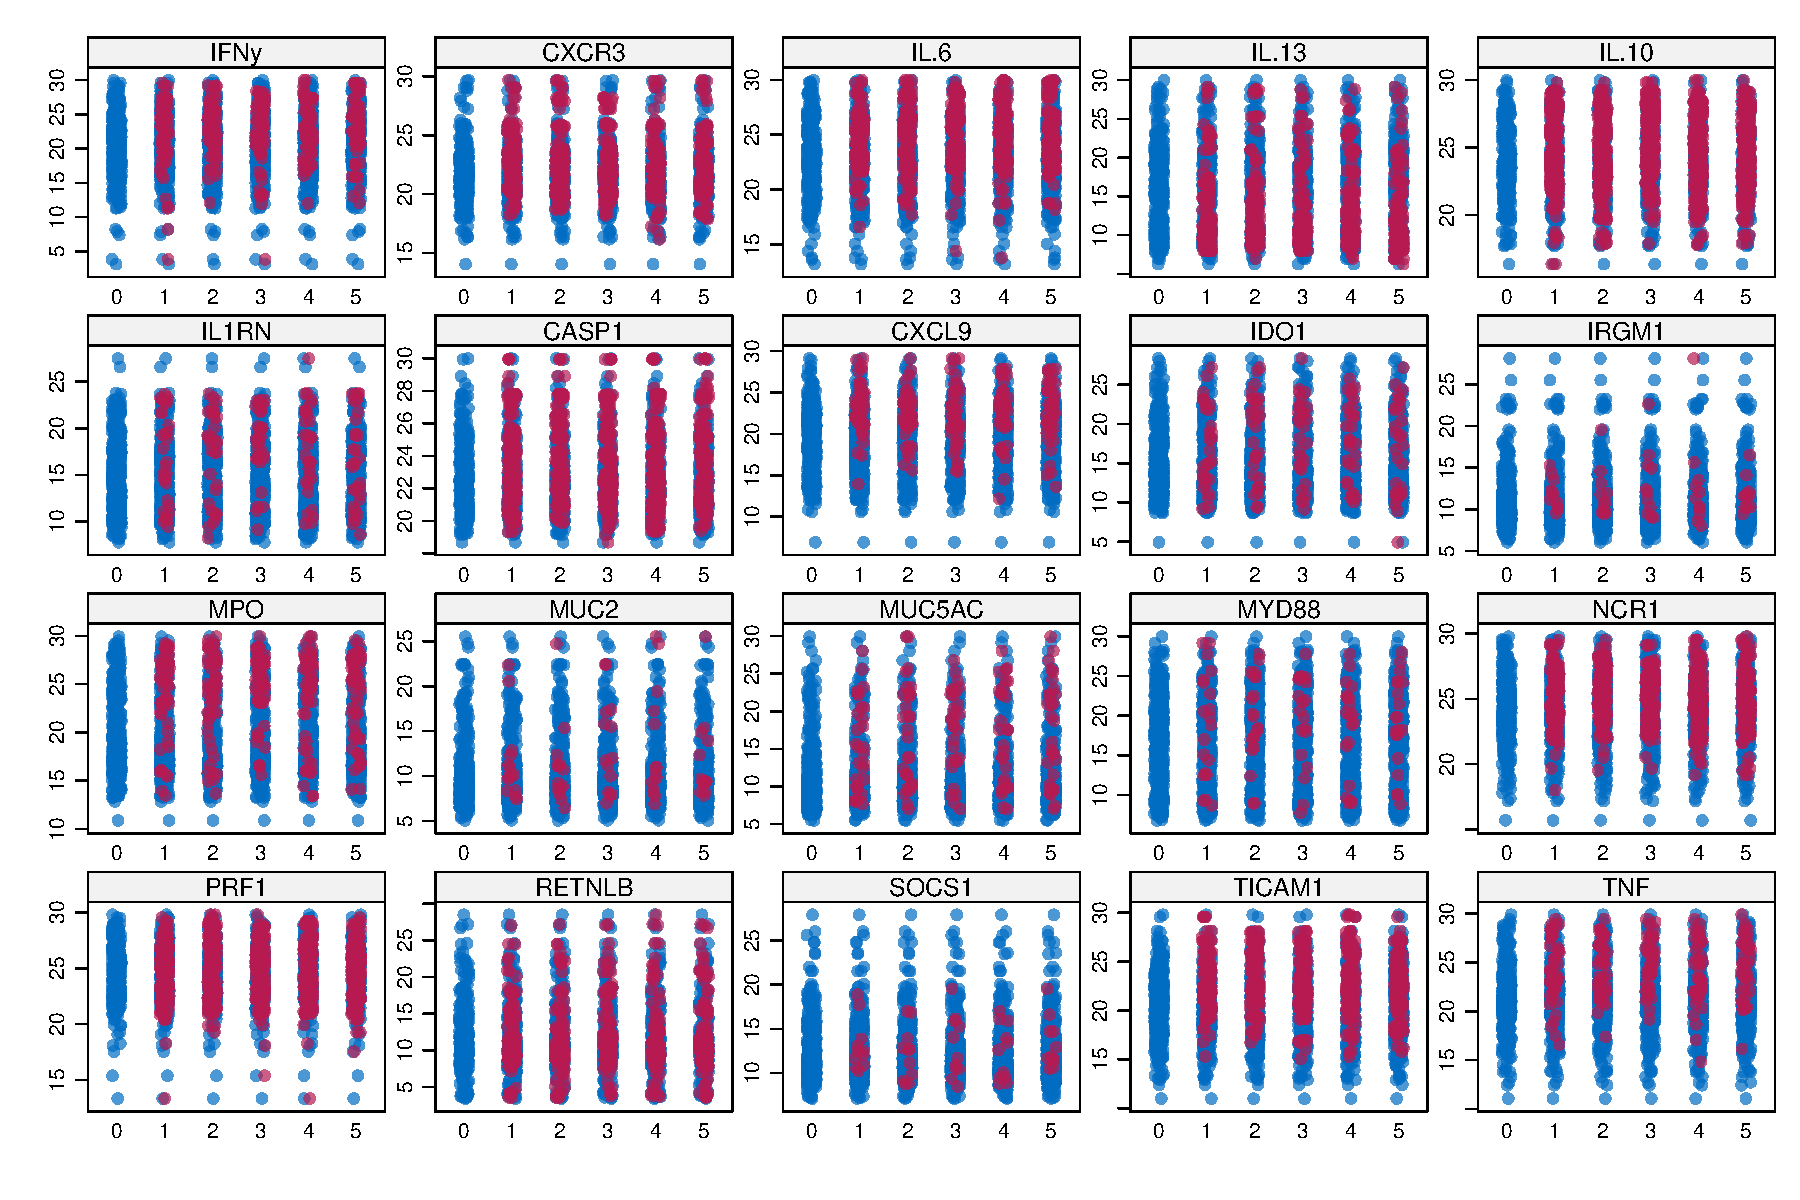
\includegraphics[width=1\linewidth]{TAC_report_2022_files/figure-latex/fig1-1} \caption{Stripplot of observed and imputed data}\label{fig:fig1}
\end{figure*}

\begin{figure*}[th]
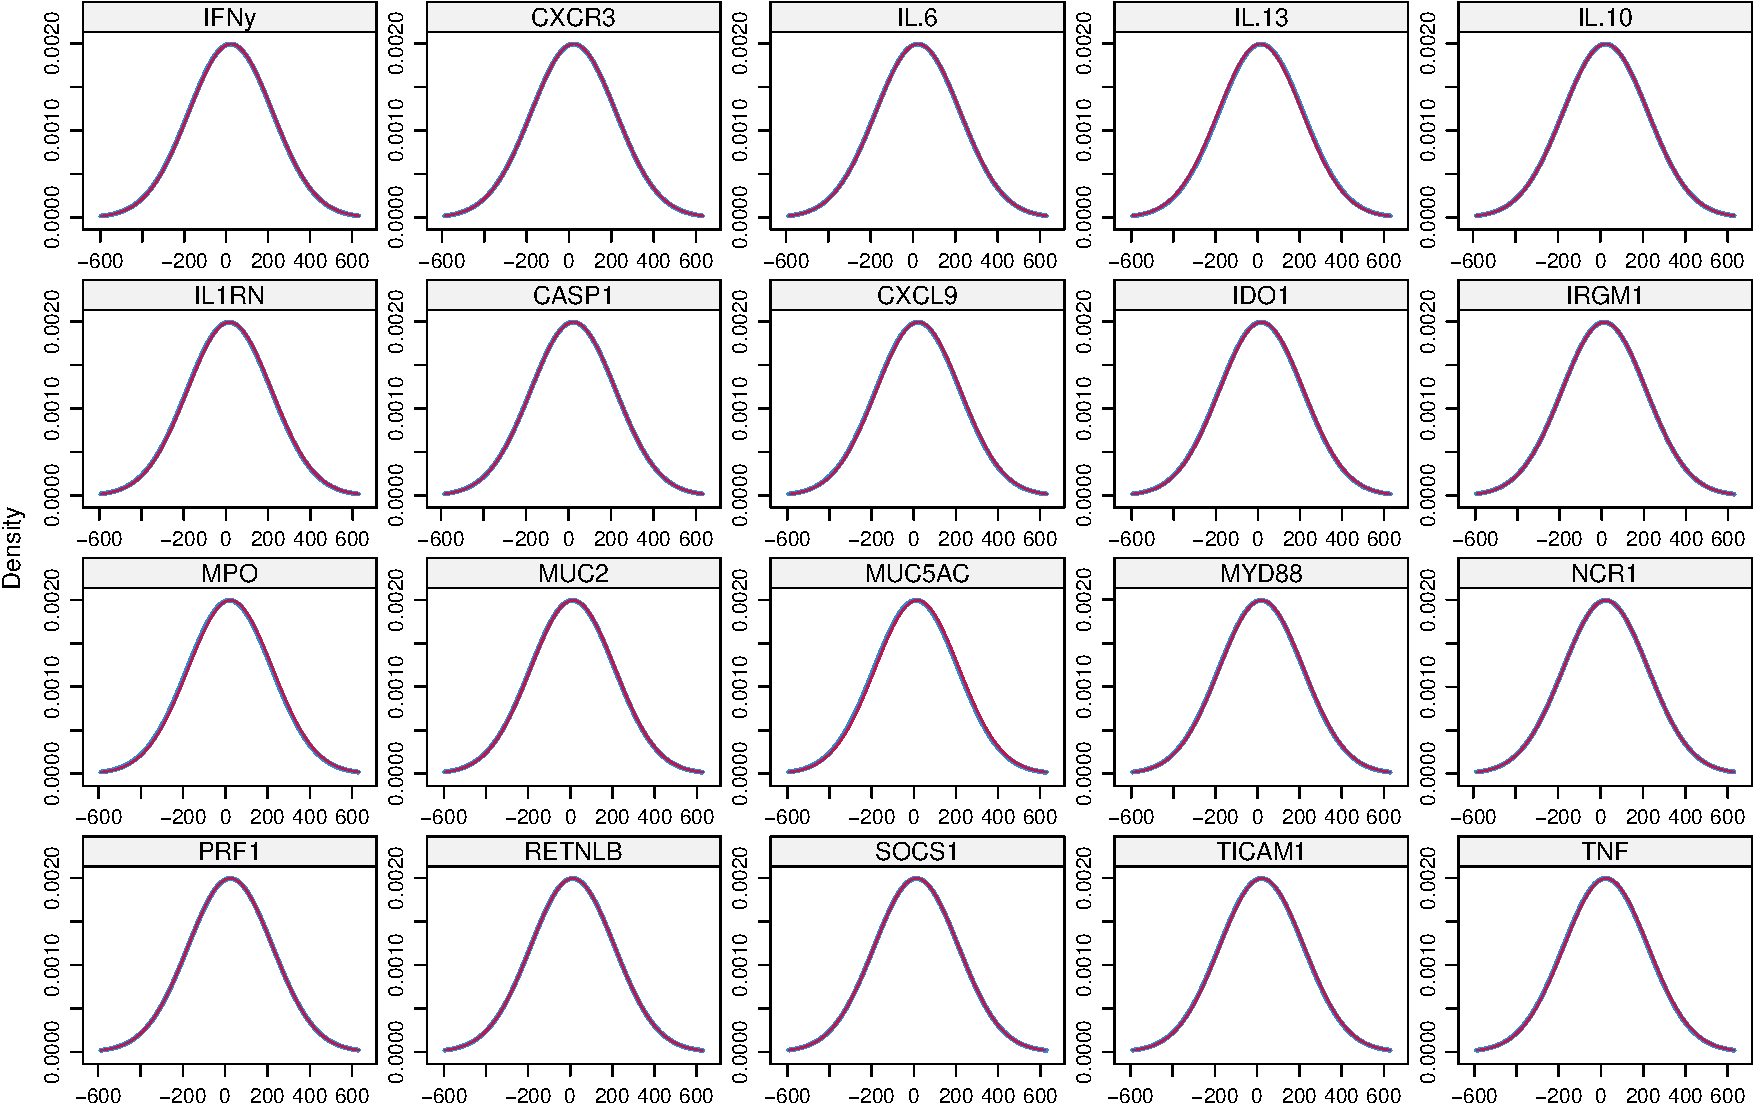
\includegraphics[width=1\linewidth]{TAC_report_2022_files/figure-latex/fig2-1} \caption{Density plot of observed and imputed data}\label{fig:fig2}
\end{figure*}

\hypertarget{questions-to-dos}{%
\paragraph{Questions / To-dos:}\label{questions-to-dos}}

\begin{enumerate}
\def\labelenumi{\arabic{enumi}.}
\tightlist
\item
  Should I log-transform the data prior to imputation?
\item
  Increasing produced data sets / iterations
\item
  sensitivity analyses using complete cases only
\end{enumerate}

\hypertarget{random-forest}{%
\subsubsection{Random forest}\label{random-forest}}

In an attempt to predict the health impact of infections in mice, we
used a random forest model Breiman (2001). We chose the maximum weight
loss during the experimental laboratory infections of mice with the
parasite \emph{Eimeria spp.} as a response variable. Maximum weight loss
is here used as a proxy describing the health impact caused by
infections. The random forest was constructed utilizing the expression
data of 20 genes, obtained by the biomarker assay (utilizing the R
package ``randomForest,'' ntree = 1000). The data set was split into a
training data set of 70 \% and to a testing data set of 30 \% to avoid
over-fitting and to assess the performance of the model on ``unseen''
data.

As a quality assessment, we used k- fold cross validation, where the
data set is divided into k subsets. Each time, the model is assessed by
using one of the k subsets as the test data set and the other as the
training data set. The model was then fitted on each k-subset and
afterwards evaluated on the test set. Last the evaluation score was
noted and the model then discarded. Further, a permutation test
cross-validation was implemented (using the function
``rf.crossValidation'' (using the R package rfUtilities, version 2.1-5).
The percent variance explained from the specified fit model was 27.7\%.
Moreover, the mean squared error from each bootstrapped model was 44.14.
Next, the variable importance was calculated according to the total
decrease in node impurities from splitting on each variable, averaged
over all trees. In this case of regression, the node impurity is
measured by residual sum of squares. Variables with comparatively higher
importance have a greater impact on the predictions of the model.

\begin{verbatim}
## running: regression cross-validation with 99 iterations
\end{verbatim}

\begin{verbatim}
## [1] 27.7
\end{verbatim}

\begin{verbatim}
## [1] 44.13772
\end{verbatim}

\begin{verbatim}
## [1] 78
\end{verbatim}

\begin{verbatim}
## [1] 6.543936
\end{verbatim}

\begin{figure*}[th]
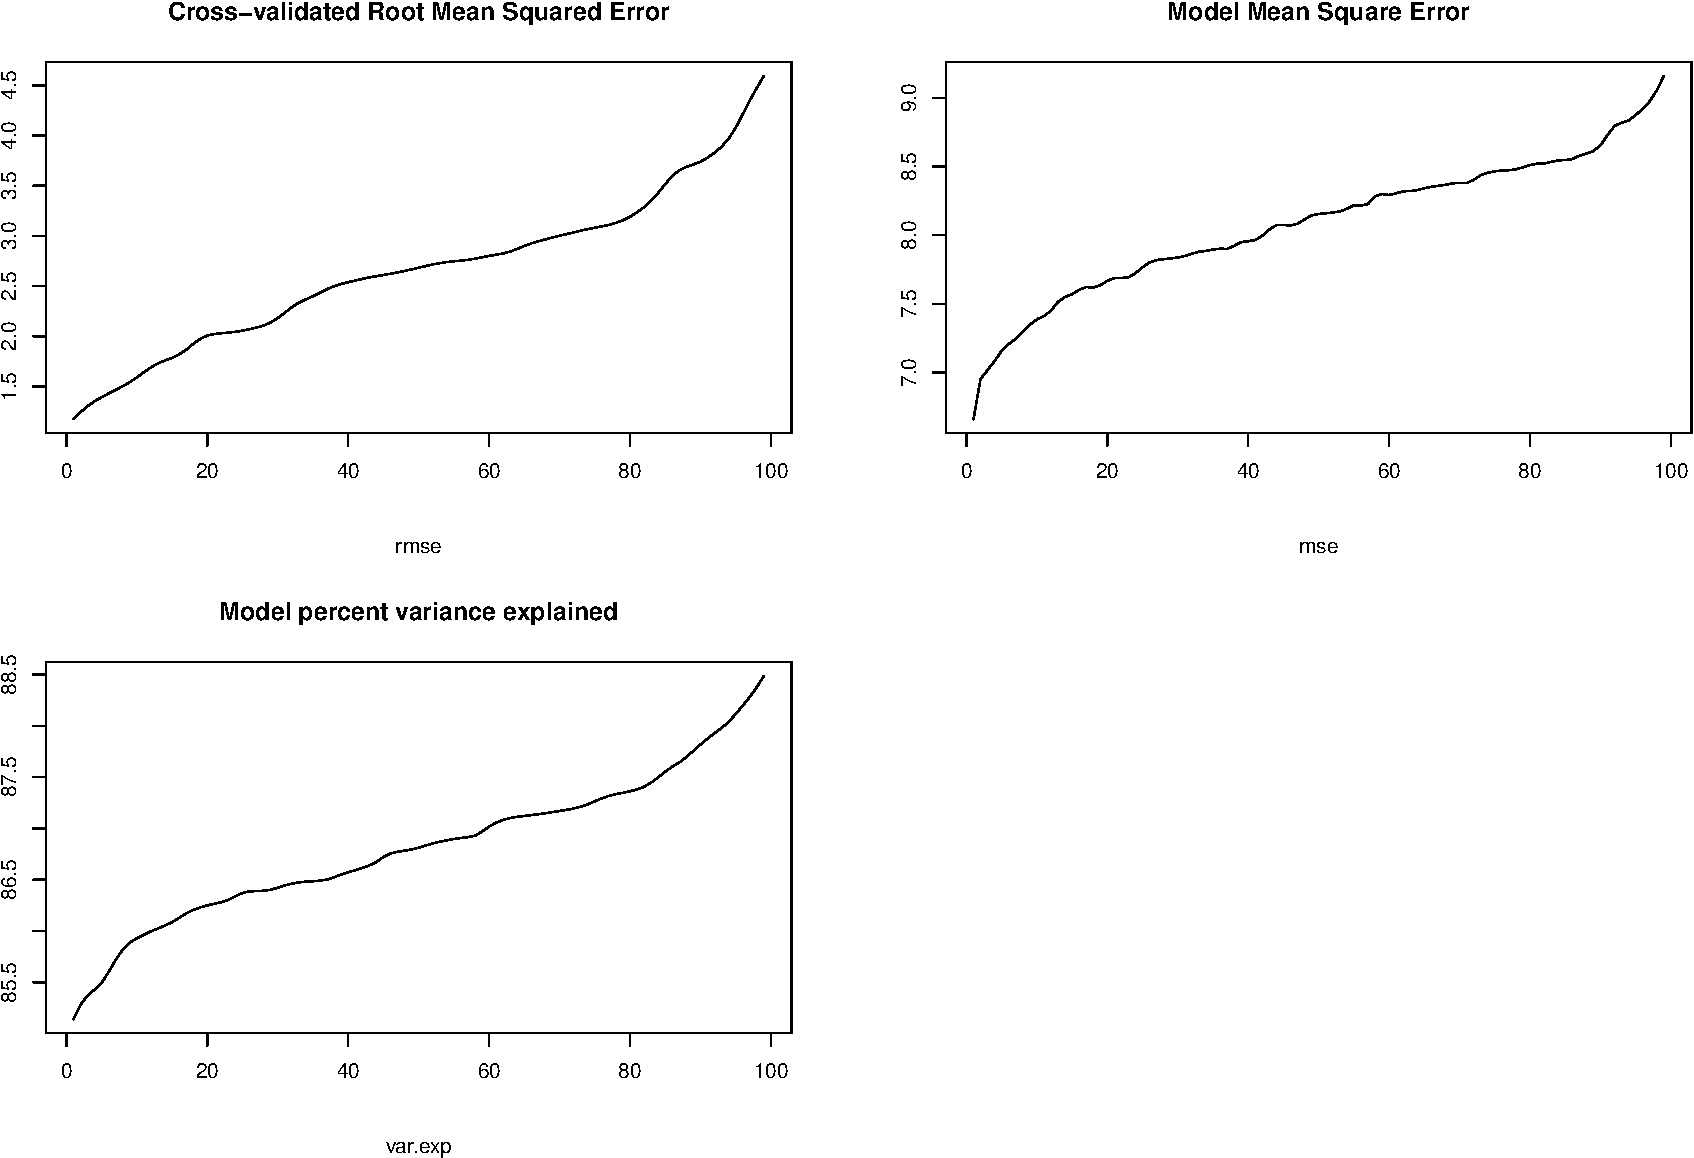
\includegraphics[width=1\linewidth]{TAC_report_2022_files/figure-latex/fig4-1} \caption{Variance explained and Root Mean Squared Error}\label{fig:fig4}
\end{figure*}

\begin{verbatim}
##        IncNodePurity Var.Names
## SOCS1       582.5419     SOCS1
## TICAM1      549.4166    TICAM1
## CXCL9       538.1206     CXCL9
## IL.6        459.0768      IL.6
## IFNy        395.9684      IFNy
## IL1RN       327.9611     IL1RN
## RETNLB      289.5686    RETNLB
## NCR1        239.8289      NCR1
## TNF         226.3735       TNF
## MPO         214.1609       MPO
## IL.13       201.9333     IL.13
## MUC2        200.2868      MUC2
## MYD88       196.5789     MYD88
## IRGM1       178.2120     IRGM1
## CASP1       170.0408     CASP1
## CXCR3       169.9418     CXCR3
## IDO1        162.3620      IDO1
## PRF1        161.2846      PRF1
## IL.10       156.3871     IL.10
## MUC5AC      149.1062    MUC5AC
\end{verbatim}

\begin{figure*}[th]
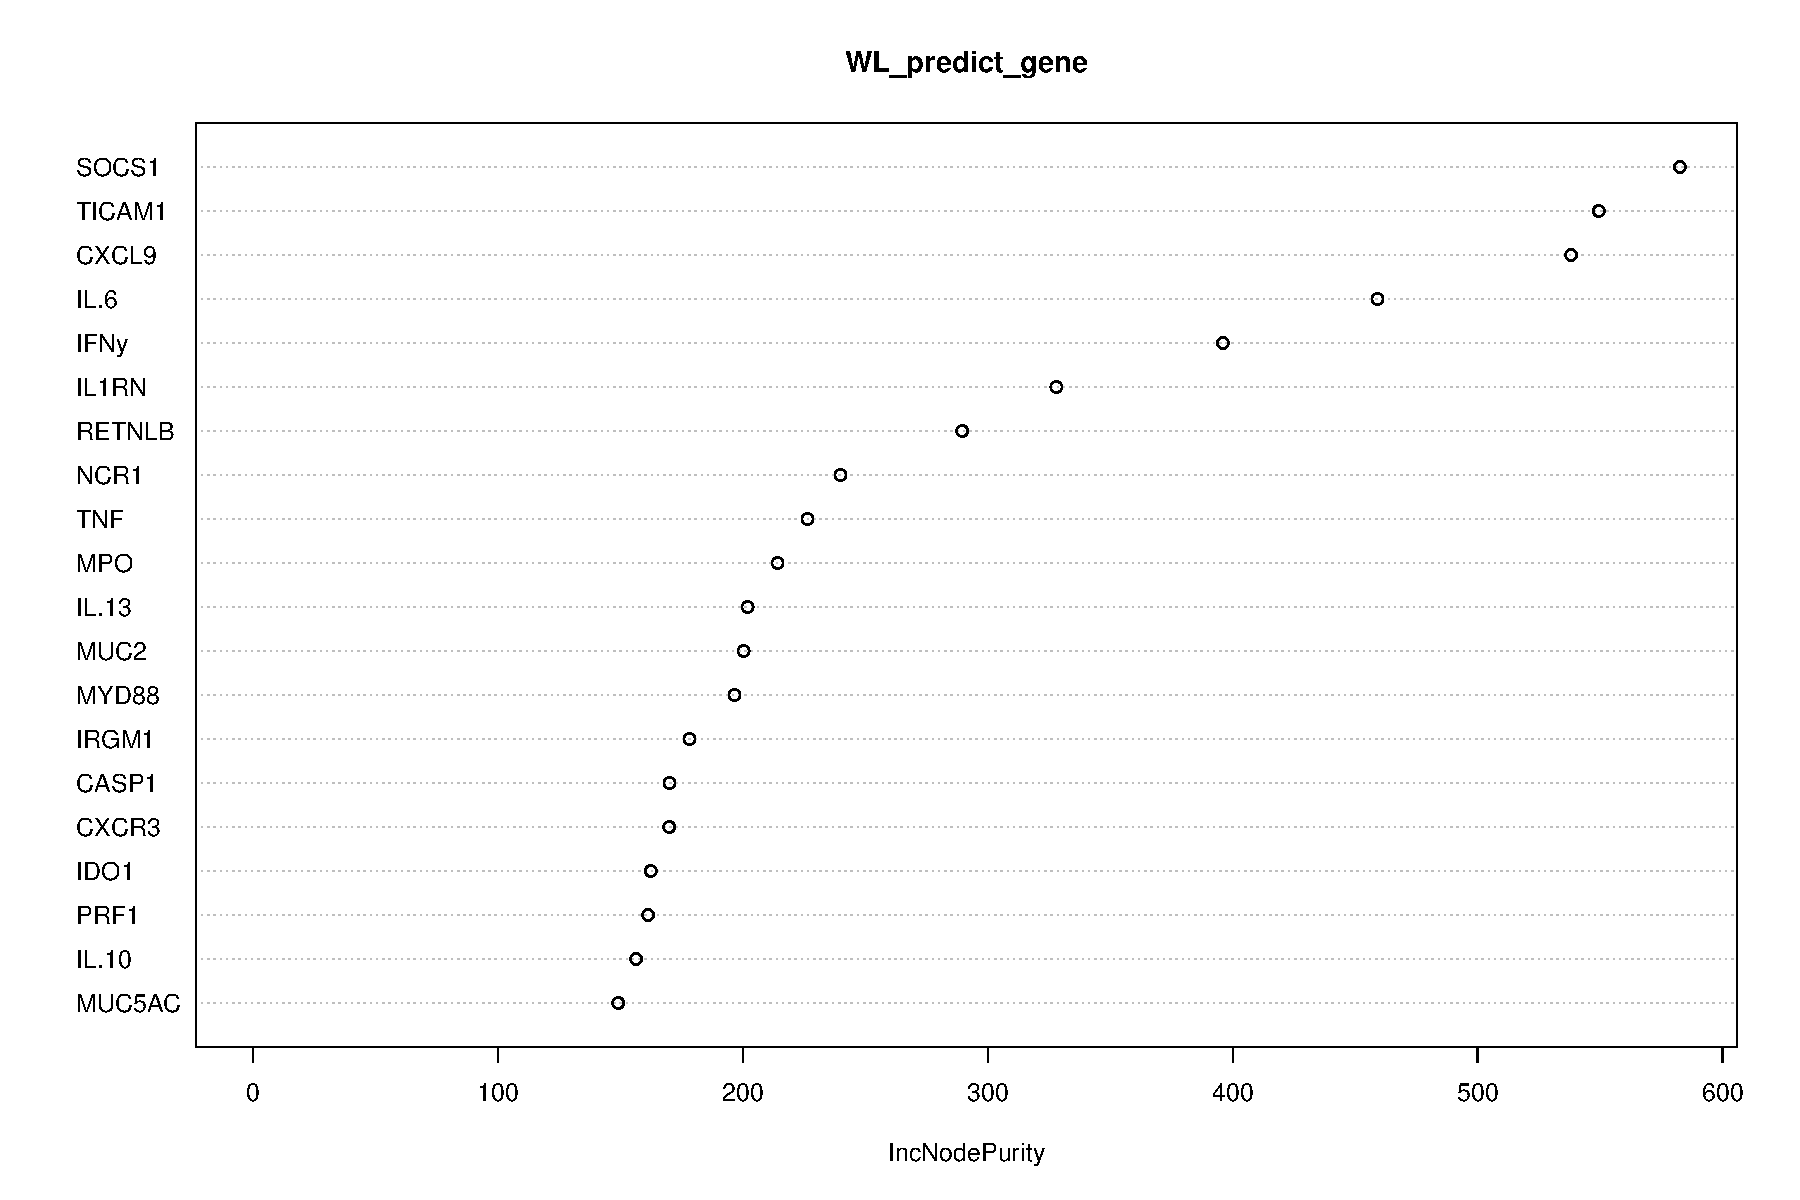
\includegraphics[width=1\linewidth]{TAC_report_2022_files/figure-latex/fig6-1} \end{figure*}

\hypertarget{results}{%
\section{Results}\label{results}}

\hypertarget{discussion}{%
\section{Discussion}\label{discussion}}

\hypertarget{conclusion}{%
\section{Conclusion}\label{conclusion}}

\hypertarget{literature-citations}{%
\section{Literature citations}\label{literature-citations}}

\hypertarget{references}{%
\section*{References}\label{references}}
\addcontentsline{toc}{section}{References}

\hypertarget{refs}{}
\begin{CSLReferences}{1}{0}
\leavevmode\vadjust pre{\hypertarget{ref-balard2020intensity}{}}%
Balard, Alice, Vı́ctor Hugo Jarquı́n-Dı́az, Jenny Jost, Iva Martincová,
L'udovı́t Ďureje, Jaroslav Piálek, Miloš Macholán, Joëlle Goüy de
Bellocq, Stuart JE Baird, and Emanuel Heitlinger. 2020. {``Intensity of
Infection with Intracellular Eimeria Spp. And Pinworms Is Reduced in
Hybrid Mice Compared to Parental Subspecies.''} \emph{Journal of
Evolutionary Biology} 33 (4): 435--48.

\leavevmode\vadjust pre{\hypertarget{ref-breiman2001random}{}}%
Breiman, Leo. 2001. {``Random Forests.''} \emph{Machine Learning} 45
(1): 5--32.

\leavevmode\vadjust pre{\hypertarget{ref-van2018flexible}{}}%
Van Buuren, Stef. 2018. \emph{Flexible Imputation of Missing Data}. CRC
press.

\leavevmode\vadjust pre{\hypertarget{ref-van2011mice}{}}%
Van Buuren, Stef, and Karin Groothuis-Oudshoorn. 2011. {``Mice:
Multivariate Imputation by Chained Equations in r.''} \emph{Journal of
Statistical Software} 45: 1--67.

\end{CSLReferences}

\end{document}
